% This LaTeX document needs to be compiled with XeLaTeX.
\documentclass[12pt]{article}
\usepackage[margin=0.8in]{geometry}
\usepackage[utf8]{inputenc}
\usepackage{graphicx}
\usepackage[export]{adjustbox}
\usepackage{amsmath}
\usepackage{amsfonts}
\usepackage{amssymb}
\usepackage[version=4]{mhchem}
\usepackage{stmaryrd}
\usepackage{bbold}
%\usepackage[fallback]{xeCJK}
\usepackage{polyglossia}
\usepackage{fontspec}
\usepackage{censor}
%\setCJKmainfont{Noto Serif CJK TC}
\graphicspath{ {../Images/} }

\usepackage{tikz}
\usepackage{amsthm}
\usepackage{tcolorbox}

\tcbuselibrary{theorems}

\definecolor{GrayCen}{HTML}{d2d2d2}
\definecolor{GrayBG}{HTML}{d9d9d9}
\definecolor{BlueDef}{HTML}{104e8b}
\definecolor{GreenProp}{HTML}{025540}
\definecolor{RedMet}{HTML}{cd5556}
\definecolor{BlackSav}{HTML}{000000}
\def\censorcolor{GrayCen}
\let\svcensorrule\censorrule
\renewcommand\censorrule[1]{%
\textcolor{\censorcolor}{\svcensorrule{#1}}}

\newtcbtheorem
  []% init options
  {definition}% name
  {Définition}% title
  {%
    colback=GrayBG,
    colframe=BlueDef,
    fonttitle=\bfseries,
  }% options
  {def}% prefix

\newtcbtheorem
  []% init options
  {proposition}% name
  {Proposition}% title
  {%
    colback=GrayBG,
    colframe=GreenProp,
    fonttitle=\bfseries,
  }% options
  {prop}% prefix

\newtcbtheorem
  []% init options
  {method}% name
  {Méthode}% title
  {%
    theorem name,
    colback=GrayBG,
    colframe=RedMet,
    fonttitle=\bfseries,
  }% options
  {met}% prefix
  
\newtcbtheorem
  []% init options
  {savoir}% name
  {Savoir-faire du chapitre}% title
  {%
    theorem name,
    colback=GrayBG,
    colframe=BlackSav,
    fonttitle=\bfseries,
  }% options
  {sav}% prefix

\newtheoremstyle{break}
  {\topsep}{\topsep}%
  {}{}%
  {\bfseries}{}%
  {\newline}{}%
\theoremstyle{break}
\newtheorem*{example}{Exemple.}
\newtheorem*{remark}{Remarque.}

\newenvironment{demo}[1][\proofname]{%
  \begin{proof}[#1]$ $\newline
}{%
  \end{proof}
}

\setmainlanguage{french}
%\setmainfont{CMU Serif}

\title{
\vspace{4em}
\centering
\tcbset{colframe=BlackSav,colback=GrayBG}
\tcbox[tikznode]{
Chapitre 1 \\ Polynômes du second degré 
}
}

\author{}
\date{}


\begin{document}
\maketitle

\tableofcontents

%\newcommand{\hideM}[1]{\colorbox{gray!50}{\phantom{$\displaystyle #1$}}}
%\newcommand{\hide}[1]{\colorbox{gray!50}{\phantom{#1}}}
\newcommand{\hideM}[1]{#1}
\newcommand{\hide}[1]{#1}


\newpage

\section{Factorisation des polynômes du second degré}
Dans tout ce chapitre, $a, b$ et $c$ désignent des réels avec $a \neq 0$.

\begin{definition}{}{}
On appelle discriminant du polynôme $a x^{2}+b x+c$ le nombre réel $\Delta$ défini par :

$$
\Delta=\hideM{b^{2}-4 a c}
$$
\end{definition}

\begin{proposition}{(admise)}{}
    On considère le polynôme du second degré $a x^{2}+b x+c \quad$ (avec $a, b, c \in \mathbb{R}$ et $a \neq 0$ ).
    
    \begin{itemize}
      \item Si $\Delta>0$, en posant $x_{1}=\hideM{\dfrac{-b+\sqrt{\Delta}}{2 a}}$ et $x_{2}=\hideM{\dfrac{-b-\sqrt{\Delta}}{2 a}}$, on a :
    \end{itemize}
    
    \hspace{10em} Pour tout $x \in \mathbb{R}, a x^{2}+b x+c=a\left(x-x_{1}\right)\left(x-x_{2}\right)$.
    
    \begin{itemize}
      \item Si $\Delta=0$, en posant $x_{0}=\hideM{-\dfrac{b}{2 a}}$, on a :
    \end{itemize}
    
    \hspace{10em} Pour tout $x \in \mathbb{R}, a x^{2}+b x+c=a\left(x-x_{0}\right)^{2}$.
    
    \begin{itemize}
      \item Si $\Delta<0, a x^{2}+b x+c$ n'est pas factorisable comme produit de deux polynômes de degré 1 .
    \end{itemize}
\end{proposition}

\section{Racines d'un polynôme du second degré}
\begin{definition}{}{}
Les solutions de l'équation $a x^{2}+b x+c=0$ sont appelées les racines du polyôme $a x^{2}+b x+c$.
\end{definition}

\begin{proposition}{}{}
On considère l'équation $a x^{2}+b x+c=0$ (avec $a, b, c \in \mathbb{R}$ et $a \neq 0$ ) où l'inconnue est $x \in \mathbb{R}$.

\begin{itemize}
  \item Si $\Delta>0$, alors l'équation admet deux solutions réelles distinctes :
\end{itemize}

$$
x_{1}=\hideM{\dfrac{-b-\sqrt{\Delta}}{2 a}} \quad \text { et } \quad x_{2}=\hideM{\dfrac{-b+\sqrt{\Delta}}{2 a}}
$$

\begin{itemize}
  \item Si $\Delta=0$, alors l'équation admet une unique solution réelle : $x_{0}=\dfrac{-b}{2 a}$.
  \item Si $\Delta<0$, alors l'équation n'admet aucune solution réelle.
\end{itemize}
\end{proposition}

\newpage
\begin{demo}
Soient $a, b, c \in \mathbb{R}$ avec $a \neq 0$.\\
Soit $x \in \mathbb{R}$. D'après la démonstration de la propriété 2 :

\begin{itemize}
  \item Si $\Delta>0$,

$$
a x^{2}+b x+c=a\left(x-x_{1}\right)\left(x-x_{2}\right) \text {. }
$$

avec $x_{1}=\dfrac{-b-\sqrt{\Delta}}{2 a}$ et $x_{2}=\dfrac{-b+\sqrt{\Delta}}{2 a}$.\\
En utilisant la règle du produit nul :

$$
\begin{aligned}
a x^{2}+b x+c=0 & \Longleftrightarrow a\left(x-x_{1}\right)\left(x-x_{2}\right)=0 \\
& \Longleftrightarrow x-x_{1}=0 \text { ou } x-x_{2}=0 \\
& \Longleftrightarrow x=x_{1} \text { ou } x=x_{2} \\
& \Longleftrightarrow x=\dfrac{-b-\sqrt{\Delta}}{2 a} \text { ou } x=\dfrac{-b+\sqrt{\Delta}}{2 a}
\end{aligned}
$$

  \item Si $\Delta=0$,
  $$
    a x^{2}+b x+c=a\left(x-x_{0}\right)^{2}
  $$
  avec $x_{0}=\dfrac{-b}{2 a}$.\\

En utilisant la règle du produit nul :

$$
\begin{aligned}
a x^{2}+b x+c=0 & \Longleftrightarrow a\left(x-x_{0}\right)^{2}=0 \\
& \Longleftrightarrow x-x_{0}=0 \\
& \Longleftrightarrow x=\dfrac{-b}{2 a}
\end{aligned}
$$

  \item On admettra que si $\Delta<0$, l'équation $a x^{2}+b x+c=0$ n'admet pas de solution.
\end{itemize}
\end{demo}

\begin{example}
Résoudre l'équation $x^{2}+x-1=0$.\\
Solution :\\
$\Delta=b^{2}-4 a c=1^{2}-4 \times 1 \times(-1)=5$. Ainsi, l'équation admet deux solutions :

$$
\begin{aligned}
& x_{1}=\dfrac{-b+\sqrt{\Delta}}{2 a}=\dfrac{-1+\sqrt{5}}{2} \\
& x_{2}=\dfrac{-b-\sqrt{\Delta}}{2 a}=\dfrac{-1-\sqrt{5}}{2}
\end{aligned}
$$
\end{example}

\begin{proposition}{Relations coefficients/racines}{}
    
Si le polynôme $a x^{2}+b x+c$ admet deux racines $x_{1}$ et $x_{2}$ (avec éventuellement $x_{1}=x_{2}$ ), alors

$$
\left\{\begin{array}{cc}
x_{1}+x_{2} & =\hideM{-\dfrac{b}{a}} \\
\text { et } & \\
x_{1} x_{2} & =\hideM{\dfrac{c}{a}}
\end{array}\right.
$$
\end{proposition}
\begin{demo}
Soit $f(x)=a x^{2}+b x+c$.\\
Comme $x_{1}$ et $x_{2}$ sont les racines de $f$, on sait que $f$ se factorise de la façon suivante : $f(x)=$ $a\left(x-x_{1}\right)\left(x-x_{2}\right)$.\\
En développant, on obtient

$$
\begin{aligned}
f(x) & =a\left(x^{2}-x_{1} x-x_{2} x+x_{1} x_{2}\right) \\
& =a x^{2}-a\left(x_{1}+x_{2}\right) x+a x_{1} x_{2}
\end{aligned}
$$

Ainsi, en identifiant les coefficients, on obtient

Par conséquent,

$$
\left\{\begin{array}{ccc}
x_{1}+x_{2} & = & -\dfrac{b}{a} \\
\text { et } & \\
x_{1} x_{2} & =\dfrac{c}{a}
\end{array}\right.
$$
\end{demo}

\begin{example}
Résoudre l'équation $x^{2}-6 x+5=0$ en commençant par remarquer que 1 est une racine «évidente».
Solution :\\
1 est une racine évidente car $1^{2}-6 \times 1+5=0$.\\
Comme on sait que le produit des racines $x_{1} \times x_{2}=5$, on en déduit que $x_{2}=\dfrac{5}{x_{1}}=5$ est la deuxième racine.
\end{example}

\newpage
\section{Signe d'un polynôme du second degré}

\begin{proposition}{}{}
Le tableau de signe de $a x^{2}+b x+c$ dépend du signe de $a$ et de $\Delta$ :\\
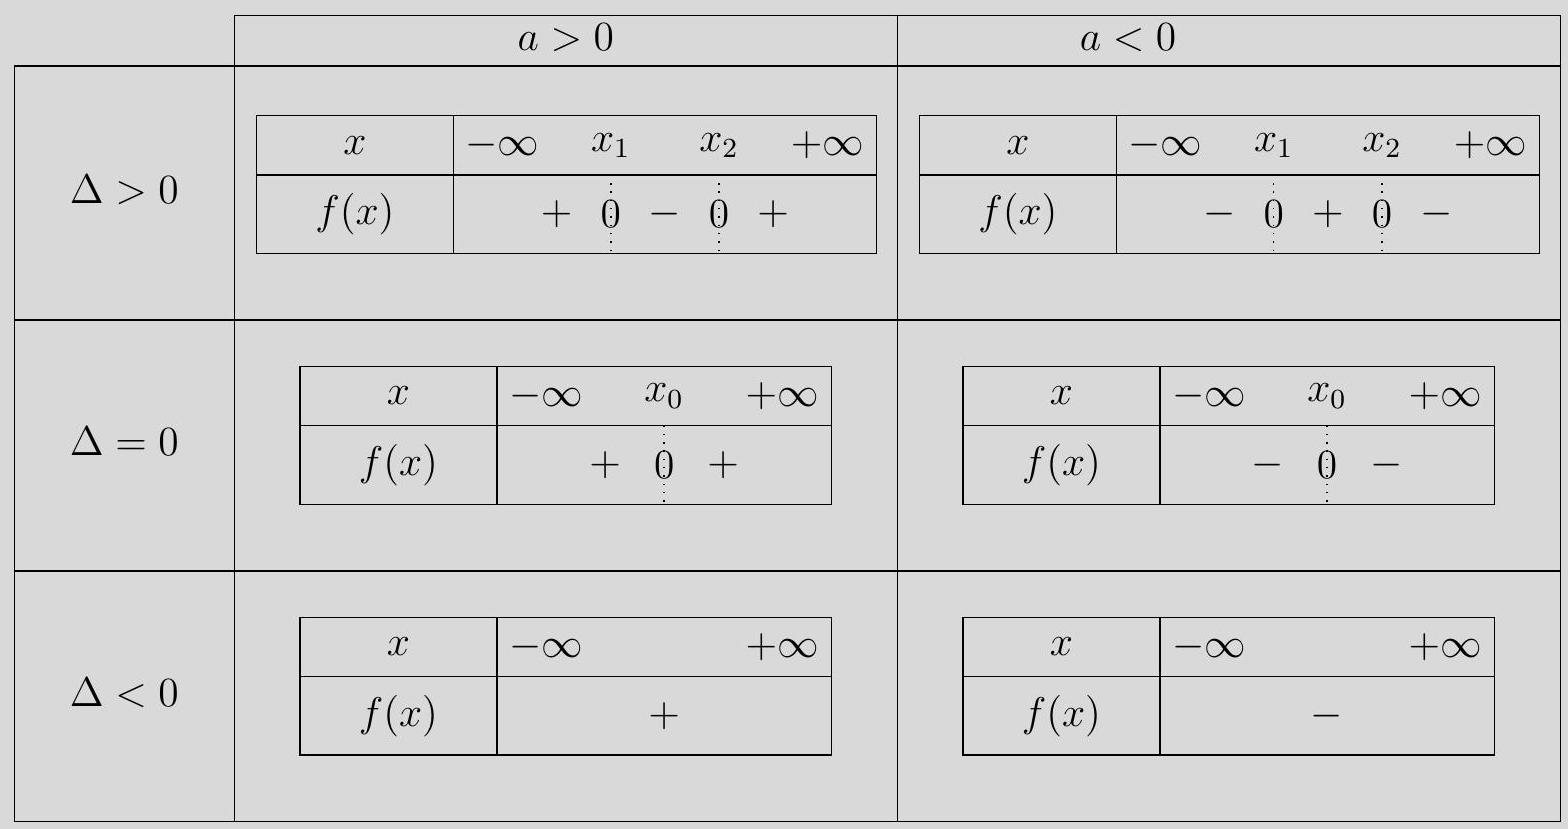
\includegraphics[max width=\textwidth, center]{2024_10_10_26b28d10fe14c9dc5e79g-05}
\end{proposition}
\begin{demo}
La démonstration découle directement de la factorisation des polynômes (propriété 2).\\
Par exemple, dans le cas où $\Delta>0$ et $a>0$ :\\
pour tout $x \in \mathbb{R}, a x^{2}+b x+c=a\left(x-x_{1}\right)\left(x-x_{2}\right)$.\\
On peut donc établir le tableau de signes suivant:

\begin{center}
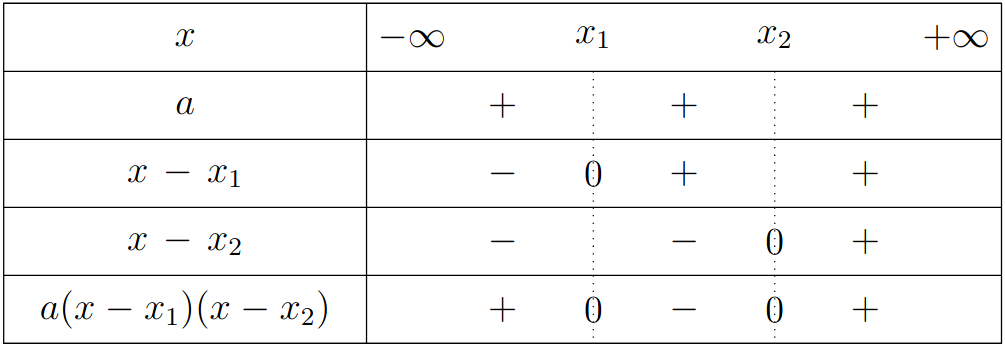
\includegraphics[width=0.6\linewidth]{Screenshot from 2024-10-23 12-47-23.png}
%\begin{tabular}{|c|cccccccl|}
%\hline
%$x$ & $-\infty$ &  & $x_{1}$ &  & $x_{2}$ &  & $+\infty$ \\
%\hline
%$a$ &  & + &  & + & $\ddots$ & + &  \\
%\hline
%$x-x_{1}$ &  & - & 0 & + &  & + &  \\
%\hline
%$x-x_{2}$ &  & - &  & - & 0 & + &  \\
%\hline
%$a\left(x-x_{1}\right)\left(x-x_{2}\right)$ &  & + & 0 & - & 0 & + &  \\
%\hline
%\end{tabular}
\end{center}
Les autres cas se traitent de la même manière.
\end{demo}

\begin{example}
Résoudre l'inéquation $2 x^{2}-5 x+1<0$.\\
Solution :\\
On cherche les racines de $2 x^{2}-5 x+1$ :\\
$\Delta=(-5)^{2}-4 \times 2 \times 1=17>0$.\\
Ainsi, les deux racines sont

$$
x_{1}=\dfrac{-b-\sqrt{\Delta}}{2 a}=\dfrac{5-\sqrt{17}}{4} \quad \text { et } x_{2}=\dfrac{-b+\sqrt{\Delta}}{2 a}=\dfrac{5+\sqrt{17}}{4}
$$

Par ailleurs, comme $a=2>0$, le tableau de signe du polynôme est le suivant :\\
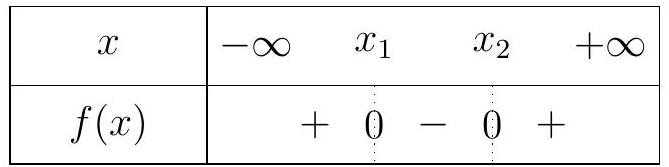
\includegraphics[max width=0.4\textwidth, center]{2024_10_10_26b28d10fe14c9dc5e79g-06}

On en déduit que l'ensemble des solutions est $\mathcal{S}=] \dfrac{5-\sqrt{17}}{4} ; \dfrac{5+\sqrt{17}}{4}[$.
\end{example}

\section{Variations d'un polynôme du second degré}
\begin{proposition}{admise}{}
    
Soit $f$ définie sur $\mathbb{R}$ par $f(x)=a x^{2}+b x+c \quad($ avec $a \neq 0)$. On pose $\alpha=\hideM{-\dfrac{b}{2 a}}$.

\begin{itemize}
  \item Si $a>0$, le tableau de variations de $f$ est :

\begin{center}
\hide{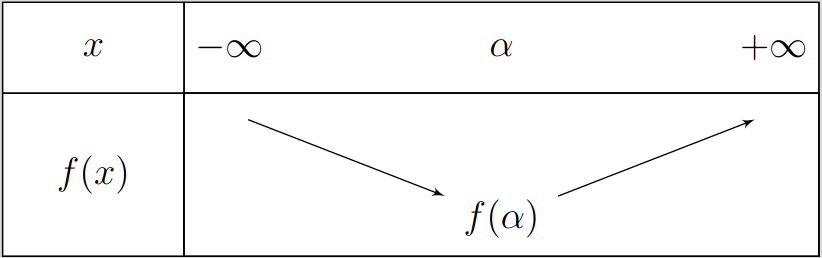
\includegraphics[width=0.5\linewidth]{Screenshot from 2024-10-23 12-56-02.png}}
\end{center}

  \item Si $a<0$, le tableau de variations de $f$ est :

\begin{center}
\hide{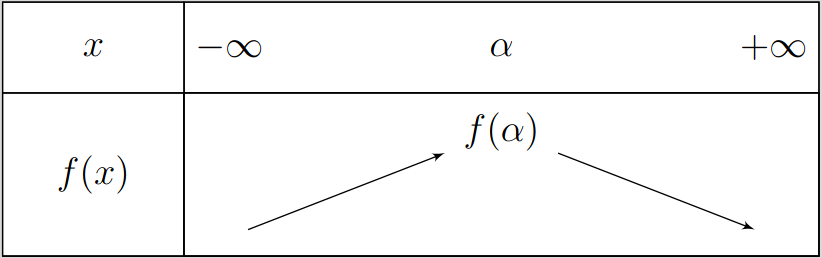
\includegraphics[width=0.5\linewidth]{Screenshot from 2024-10-23 12-56-29.png}}
\end{center}
\end{itemize}
\end{proposition}

\begin{example}
Soit $f$ définie sur $\mathbb{R}$ par $f(x)=x^{2}-3 x+4$. Déterminer les variations de $f$.\\
Solution :\\
On a $\quad \alpha=-\dfrac{b}{2 a}=-\dfrac{-3}{2 \times 1}=\dfrac{3}{2}$.\\
De plus, $f(\alpha)=\left(\dfrac{3}{2}\right)^{2}-3 \times\left(\dfrac{3}{2}\right)+4=\dfrac{7}{4}$.\\
Ainsi, comme $a=1>0$, le tableau de variations de $f$ est:
\begin{center}
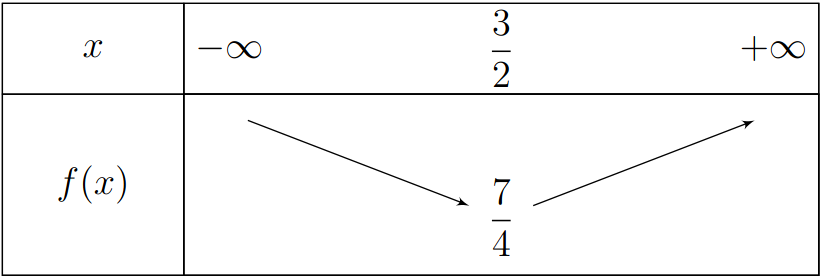
\includegraphics[width=0.5\linewidth]{Screenshot from 2024-10-23 12-58-37.png}
\end{center}
\end{example}

\newpage
\begin{definition}{}{}
    Le point de coordonnées $\hideM{(\alpha ; f(\alpha))}$ est appelé le sommet de la parabole représentative de la fonction $f$.
\end{definition}

\begin{example}
Si $f$ est définie sur $\mathbb{R}$ par $f(x)=x^{2}-3 x+4$, le point $M\left(\dfrac{3}{2} ; \dfrac{7}{4}\right)$ est le sommet de la parabole.
\end{example}

\begin{remark}
    On peut résumer la situation des racines et du signe d'un polynôme du second degré par le tableau suivant :
    
\begin{center}
\begin{tabular}{|c|c|c|}
\hline
 & $a>0$ & $a<0$ \\
\hline
$\Delta>0$ (deux racines) & 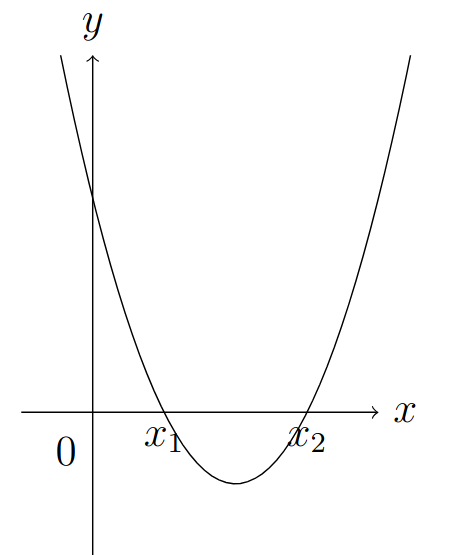
\includegraphics[max width=0.25\textwidth]{Screenshot from 2024-10-23 13-00-58.png}
 & 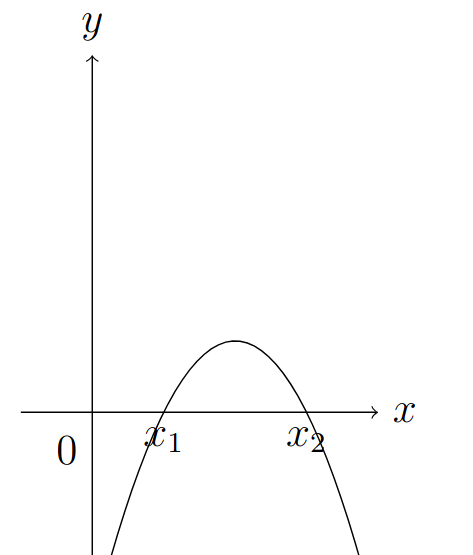
\includegraphics[max width=0.25\textwidth]{Screenshot from 2024-10-23 13-01-08.png}
 \\
\hline
$\Delta=0$ (une racine) & 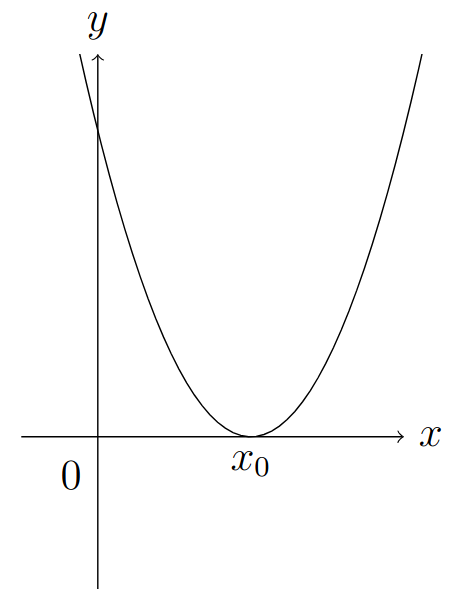
\includegraphics[max width=0.25\textwidth]{Screenshot from 2024-10-23 13-01-28.png}
 & 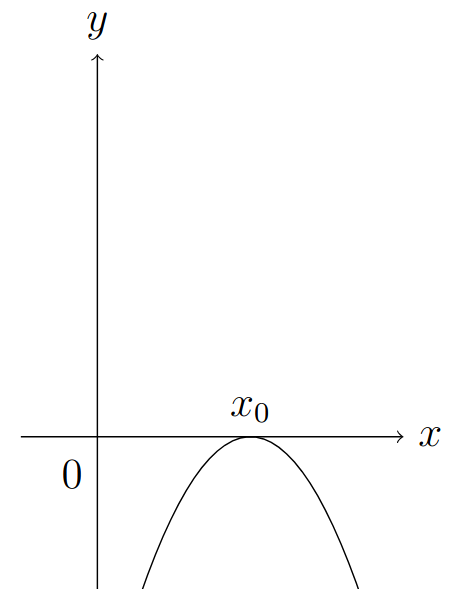
\includegraphics[max width=0.25\textwidth]{Screenshot from 2024-10-23 13-01-42.png}
 \\
\hline
$\Delta<0$ (pas de racine) & 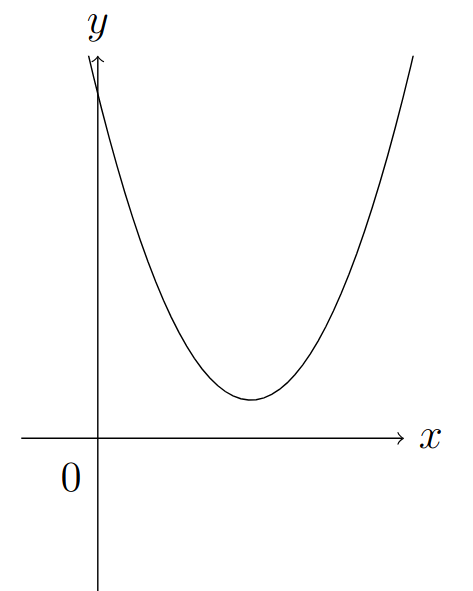
\includegraphics[max width=0.25\textwidth]{Screenshot from 2024-10-23 13-02-01.png}
 & 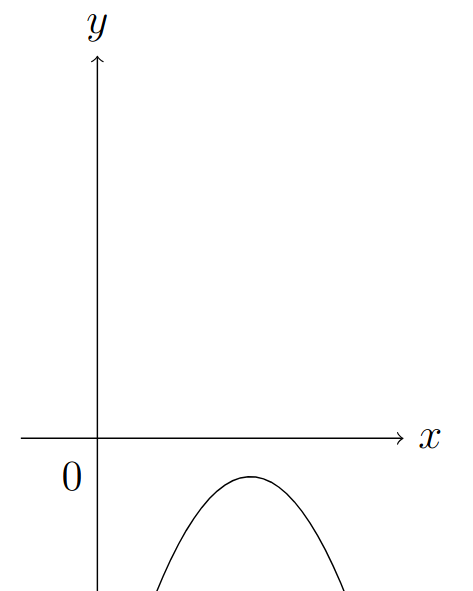
\includegraphics[max width=0.25\textwidth]{Screenshot from 2024-10-23 13-02-14.png}
 \\
\hline
\end{tabular}
\end{center}
\end{remark}

\section{Complément sur les équations de degré supérieur}
\subsection{Équations de degré 3}
La résolution générale des équations de degré 3 n'est pas au programme de première. En revanche, il est possible de résoudre une équation de degré 3 lorsqu'on connaît déjà une des solutions.

\begin{method}{Résoudre une équation de degré 3 de la forme $a x^{3}+b x^{2}+c x+d=0$}{}
    
\begin{itemize}
  \item Déterminer une racine ``évidente'' $x_{1}$.
  \item Chercher des réels $a, b, c$ tels que
\end{itemize}

$$
\hideM{a x^{3}+b x^{2}+c x+d=\left(x-x_{1}\right)\left(a x^{2}+b x+c\right)}
$$

\begin{itemize}
  \item Pour trouver $u, v, w$, développer le produit et on identifie les coefficients termes à termes des deux polynômes.
  \item Finir la résolution en résolvant $a x^{2}+b x+c=0$.
\end{itemize}
\end{method}

\begin{example}
Résoudre l'équation (E) : $x^{3}+4 x^{2}-5=0$.

Solution :\\
1 est une racine évidente.\\
On va donc factoriser l'équation par $(x-1)$, c'est-à-dire qu'on cherche $u, v, w \in \mathbb{R}$ tels que

$$
x^{3}+x^{2}-2=(x-1)\left(a x^{2}+b x+c\right)
$$

Or,

$$
\begin{aligned}
(x-1)\left(a x^{2}+b x+c\right) & =a x^{3}+b x^{2}+c x-a x^{2}-b x-c \\
& =a x^{3}+(b-a) x^{2}+(c-b) x-c
\end{aligned}
$$

En identifiant les coefficients, on obtient le système suivant :

En résolvant le système, on trouve : $a=1, b=5$ et $c=5$.\\
Ainsi, pour tout $x \in \mathbb{R}, x^{3}+x^{2}-2=(x-1)\left(x^{2}+5 x+5\right)$. On a donc

$$
\begin{aligned}
x^{3}+x^{2}-2=0 & \Longleftrightarrow(x-1)\left(x^{2}+5 x+5\right)=0 \\
& \Longleftrightarrow x-1=0 \quad \text { ou } \quad x^{2}+5 x+5=0
\end{aligned}
$$

On calcule le discriminant de $x^{2}+5 x+5: \Delta=5$.\\
Les deux solutions de $x^{2}+5 x+5=0$ sont donc $x_{1}=\dfrac{-5+\sqrt{5}}{2}$ et $x_{2}=\dfrac{-5-\sqrt{5}}{2}$.\\
Finalement, l'ensemble des solutions de (E) est :

$$
\mathcal{S}=\left\{1 ; \dfrac{-5+\sqrt{5}}{2} ; \dfrac{-5-\sqrt{5}}{2}\right\}
$$
\end{example}

\subsection{Équations de degré 4}
La résolution générale des équations de degré 4 n'est pas au programme de première. En revanche, il est possible de résoudre une équation dans un cas particulier : celui d'une équation bicarrée.

\begin{method}{Résoudre une équation de degré 4 de la forme $a x^{4}+b x^{2}+c=0$ (équation bicarrée)}{}
\begin{itemize}
  \item Poser $y=\hideM{x^{2}}$
  \item Résoudre l'équation $\hideM{a y^{2}+b y+c=0}$
  \item En déduire les racines de l'équation bicarrée.
\end{itemize}
\end{method}

\begin{example}
    Résoudre l'équation (E) : $x^{4}-x^{2}-2=0$.

Solution :\\
Soit $x \in \mathbb{R}$. On pose $y=x^{2}$.\\
On a l'équivalence :

$$
x^{4}-x^{2}-1=0 \Longleftrightarrow y^{2}-y-1=0
$$

On résout l'équation $y^{2}-y-1=0$ :\\
$\Delta=5$. L'équation admet deux solutions : $y_{1}=\dfrac{1+\sqrt{5}}{2}$ et $y_{2}=\dfrac{1-\sqrt{5}}{2}$.\\
Ainsi,

$$
\begin{aligned}
& x^{4}-x^{2}-1=0 \Longleftrightarrow\left\{\begin{array}{l}
x^{2}=\dfrac{1+\sqrt{5}}{2} \\
\text { ou } \\
x^{2}=\dfrac{1-\sqrt{5}}{2} \quad \text { (impossible) }
\end{array}\right. \\
& \Longleftrightarrow x^{2}=\dfrac{1+\sqrt{5}}{2} \\
& \Longleftrightarrow\left\{\begin{array}{l}
x=\sqrt{\dfrac{1+\sqrt{5}}{2}} \\
\text { ou } \\
x=-\sqrt{\dfrac{1+\sqrt{5}}{2}}
\end{array}\right.
\end{aligned}
$$

Finalement, l'ensemble des solutions de $(E)$ est $\mathcal{S}=\left\{\sqrt{\dfrac{1+\sqrt{5}}{2}} ;-\sqrt{\dfrac{1+\sqrt{5}}{2}}\right\}$.
\end{example}

\newpage
\begin{savoir}{}{}

\begin{itemize}
  \item Résoudre une équation du second degré en diversifiant les stratégies : discriminant, identités remarquables, racines évidentes, formule de la somme et du produit des racines.
  \item Factoriser une fonction polynôme du second degré.
  \item Déterminer le signe d'une fonction polynôme du second degré.
  \item Déterminer les variations d'une fonction polynôme du second degré.
  \item Résoudre une équation de degré 3 lorsque l'on connaît une racine évidente.
  \item Résoudre une équation bicarrée (de degré 4).
  \item Déterminer une fonction polynôme du second degré passant par trois points donnés du plan.
\end{itemize}

\end{savoir}

\end{document}